\documentclass[pdf]{beamer}
\mode<presentation>{}

\usetheme{metropolis}

\usepackage[francais]{babel}
\usepackage[utf8]{inputenc}
\usepackage[T1]{fontenc}
\usepackage{amsmath}
\usepackage{listings}
\usepackage{multimedia}
\usepackage{url}

\newcommand\gr{\selectlanguage{greek}}
\newcommand\fr{\selectlanguage{francais}}

\addtobeamertemplate{footline}{\insertframenumber/\inserttotalframenumber}

%% preamble

\title{Fouine 3.0}
\subtitle{Elles sont dans nos campagnes, dans nos villes... Elles sont sur les réseaux sociaux... }
\author{Bethune Louis, Felderhoff Joël}

%%document

\begin{document}

\begin{frame}
\titlepage
\end{frame}

\begin{frame}{La récursivité}
\begin{figure}
\center
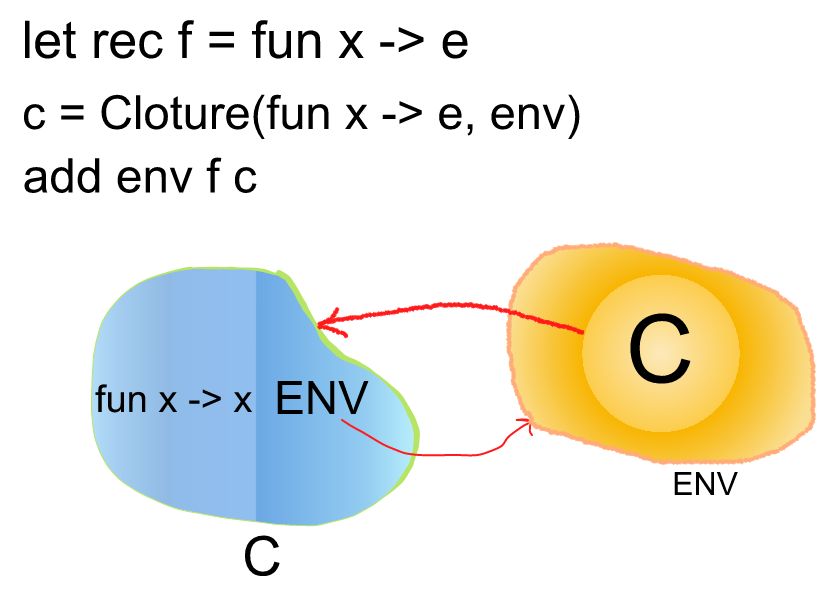
\includegraphics[scale=0.3]{Drawing.png} 
\caption {Phagocytose d'une clôture par une table de hachage}
\end{figure}
\end{frame}

\end{document}

